The proposed competition is a regression problem about age estimating; in fact, based on vocal recordings and some information regarding the person, such as his ethnicity and his gender, we aim to correctly determine the age of the person who is talking.
The data set is divided into two parts:
\begin{itemize}
    \item a \emph{development} set, containing $2933$ elements, each of them labelled  
    \item an \emph{evaluation} set, containing $691$ elements
\end{itemize}
The development set will be used to build a regressor and the estimate will be done on the evaluation set.

We can make some considerations based on the development set. First, the dataset is complete, indeed none of the rows contains missing values. 
Second, the dataset also contains the path to the vocal recordings from which we have decided to extract more features from the spectrogram.
Third, the sample rate is the same for all the audio recordings.

To better understand the distribution of the features we can plot some histograms.
From the histograms shown in figure $\eqref{hist_distributivi}$ we can notice that most of the features seems to be distributed as Gaussian distribution with not many outliers. 
Some exceptions are \textit{max\_pitch}, \textit{min\_pitch} and \textit{num\_characters}: the first two features mentioned have a very wide range of values but almost all their distribution mass is concentrated in a single point, thus there are many outliers; on the contrary, \textit{num\_characters} concentrates his mass distribution in two far values.

\begin{figure}
    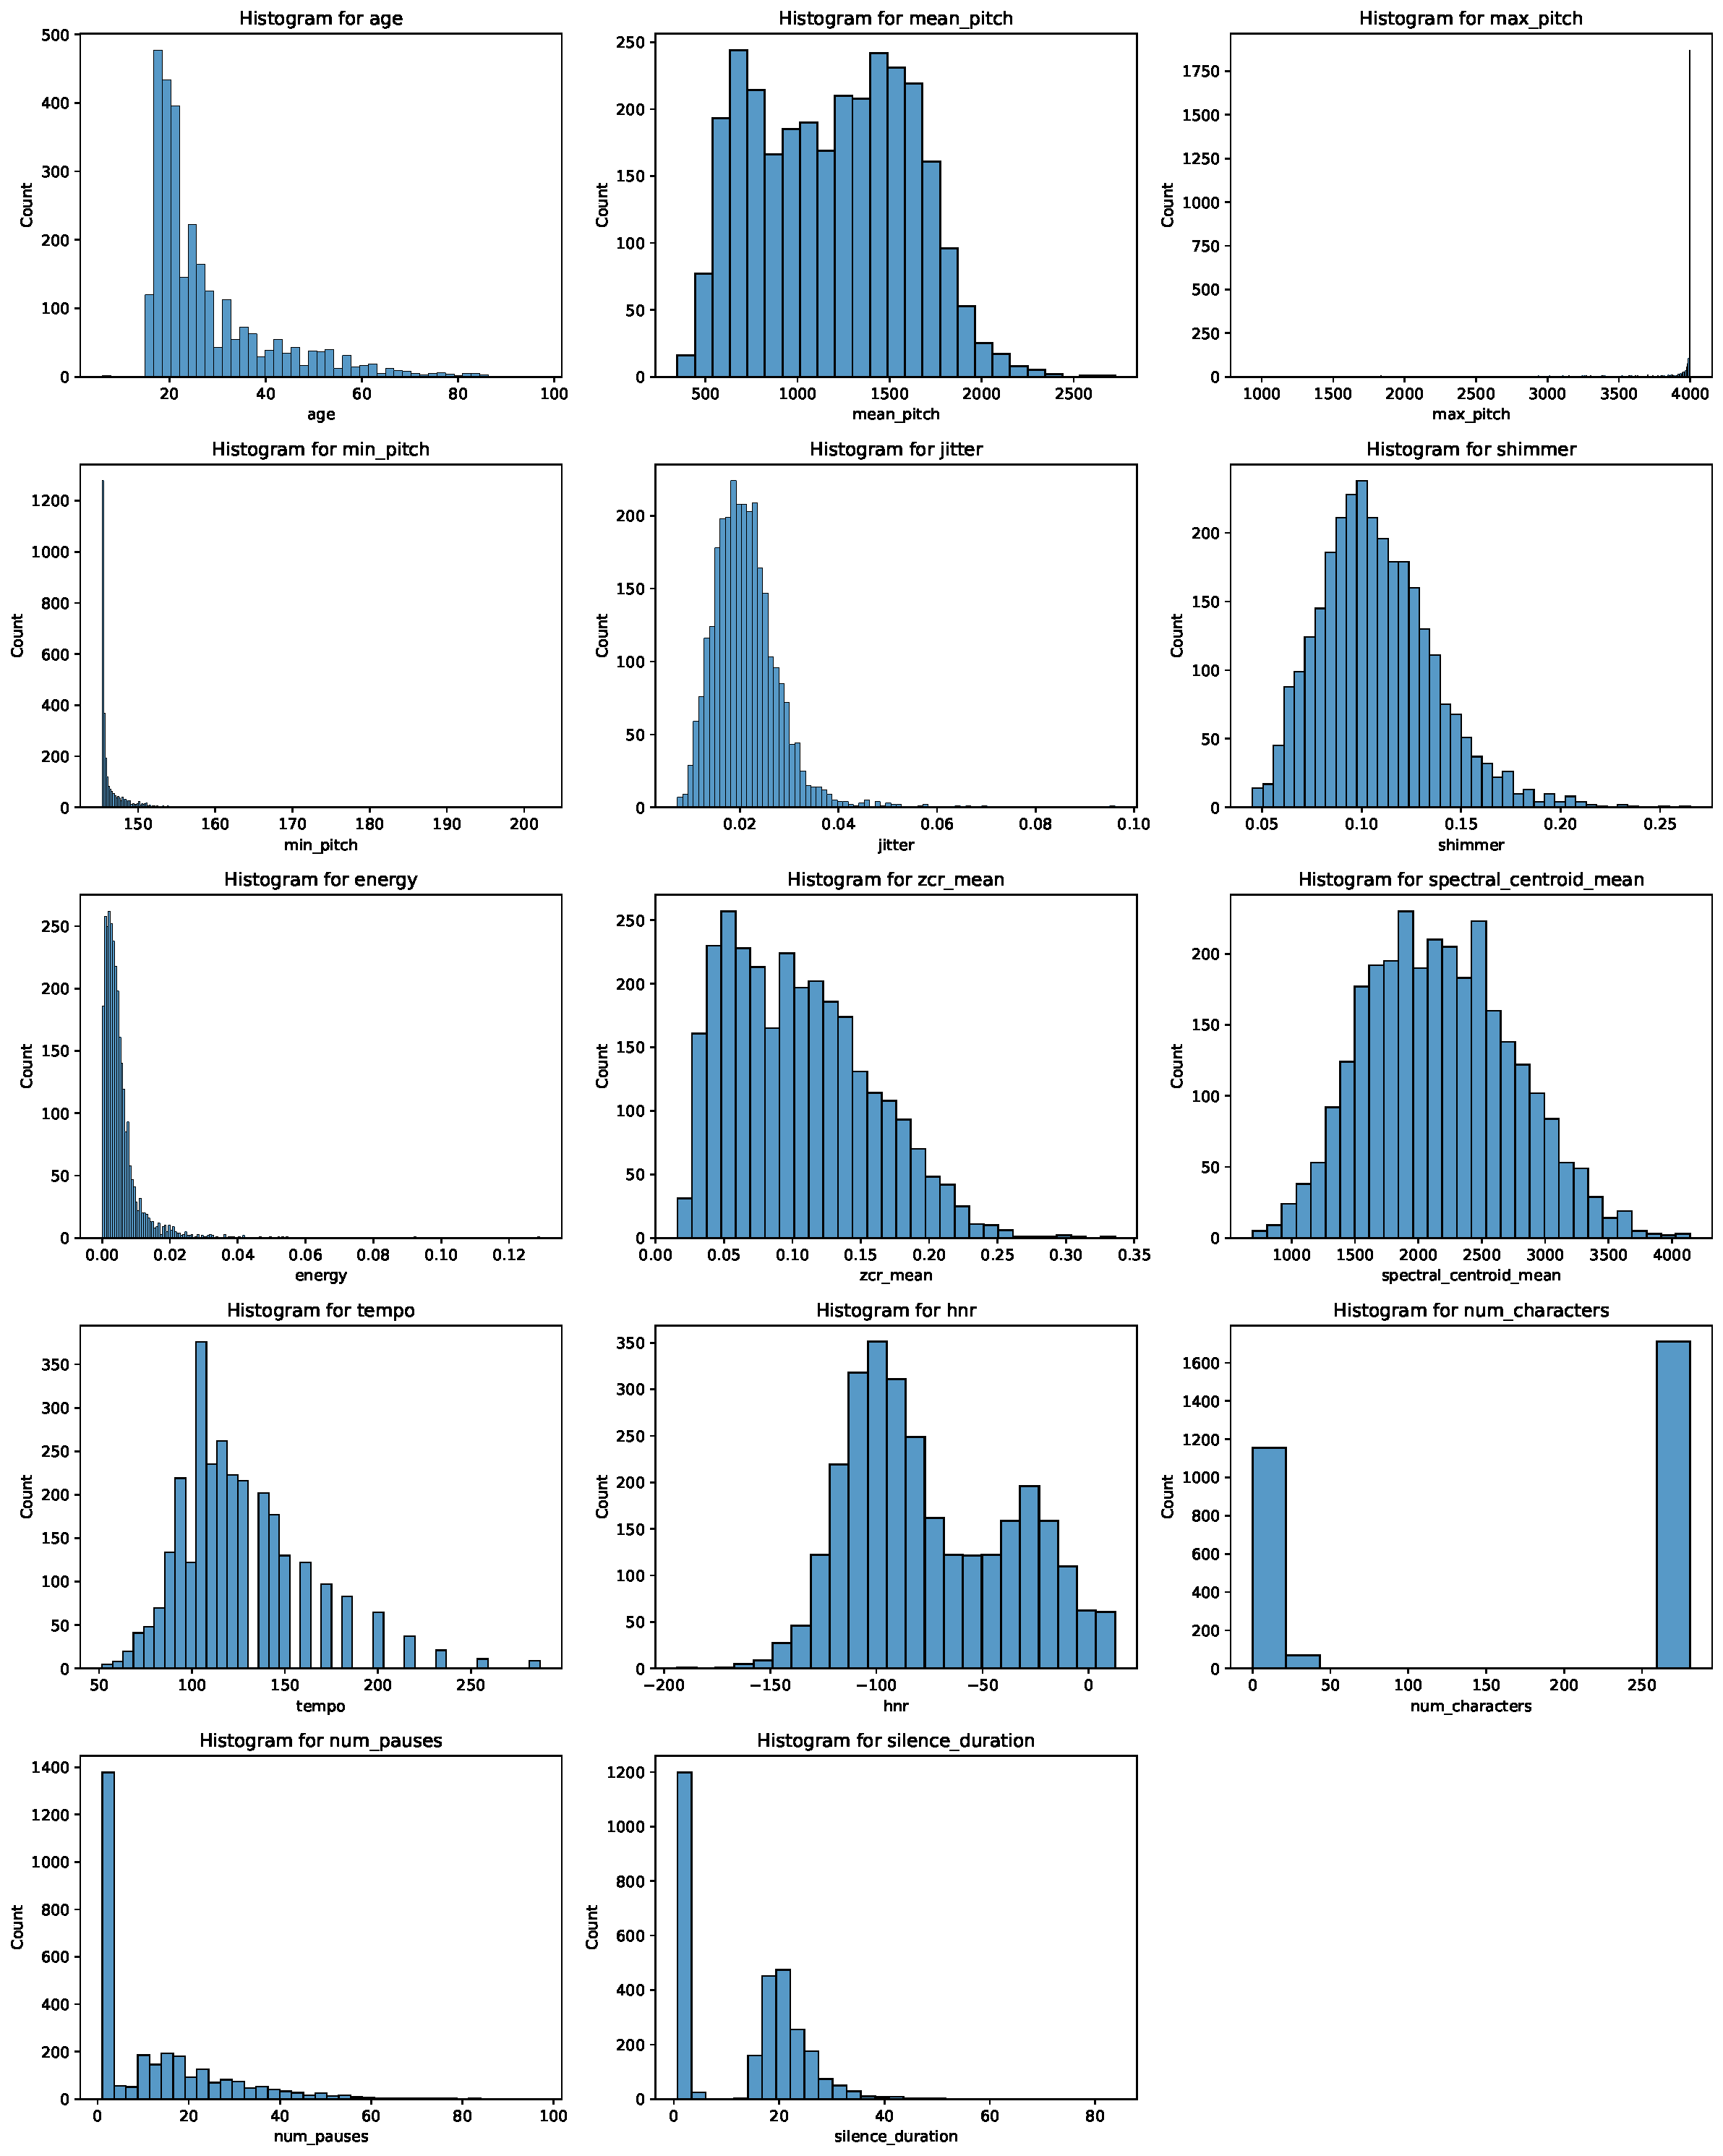
\includegraphics[width = 0.40\textwidth]{img/distribution.pdf}
    \caption{Histograms of some features.}
    \label{hist_distributivi}
\end{figure}

Another useful tool is the correlation plot shown in figure \eqref{correlation_plot}: from this plot we can spot that many features are highly correlated and this may yield redundancy into the dataset.
\begin{figure}
    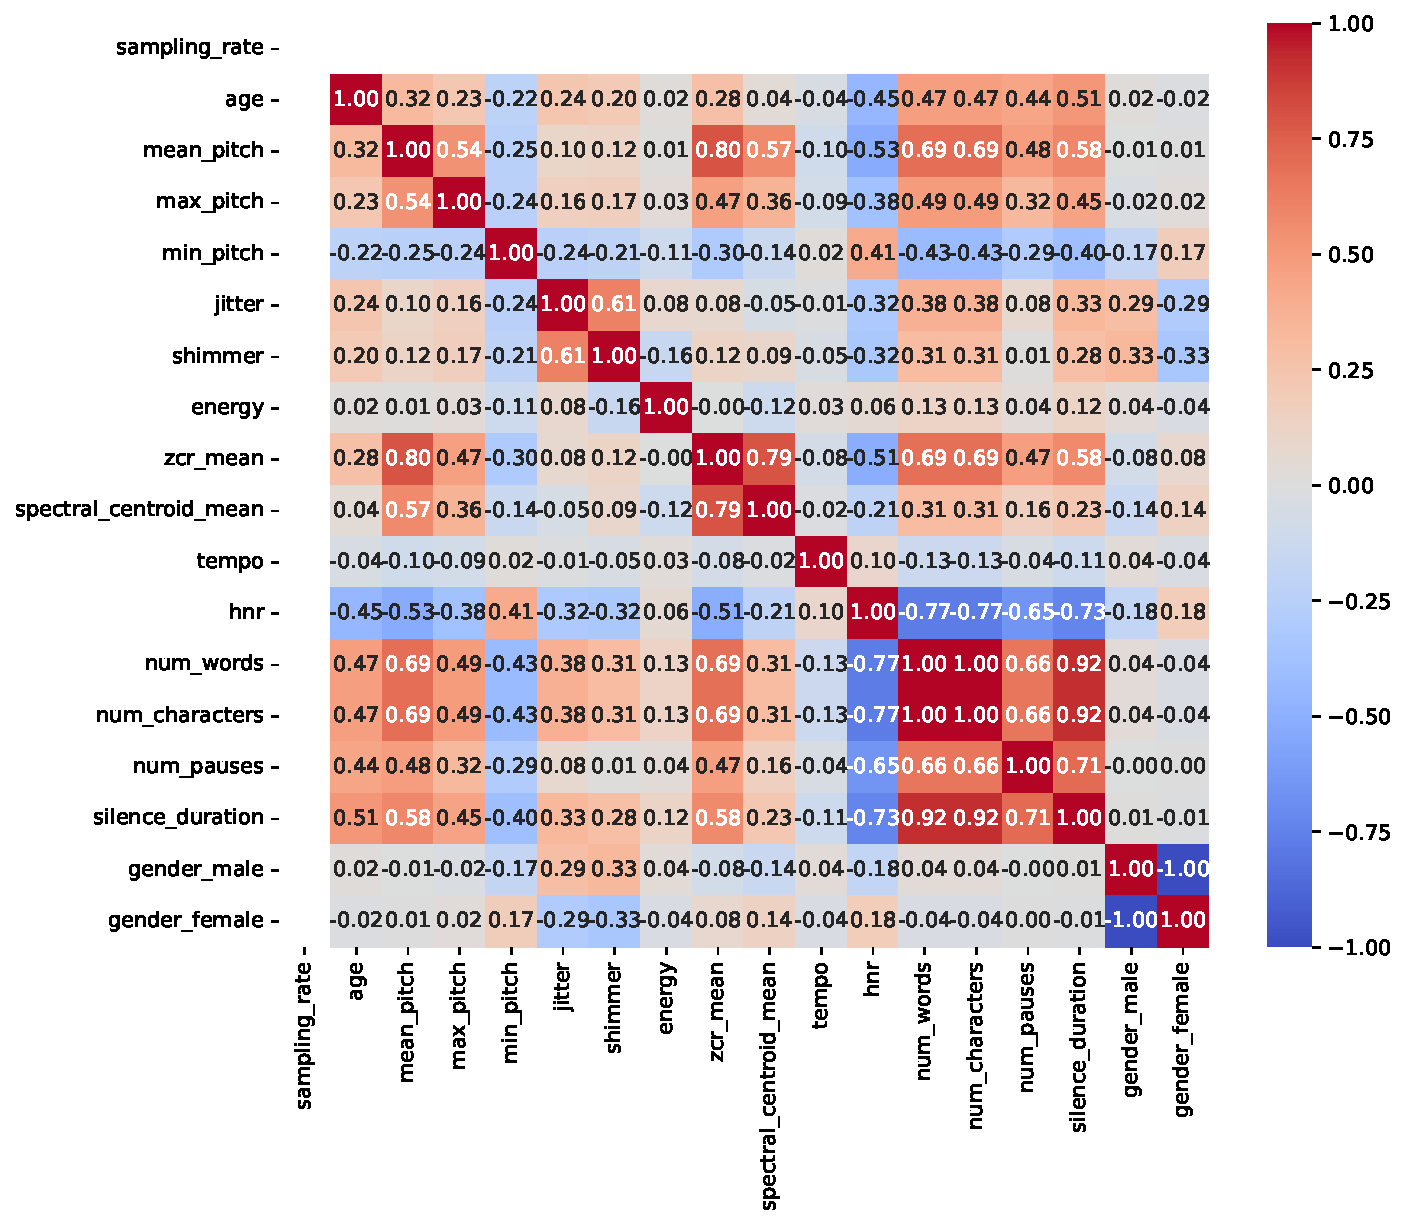
\includegraphics[width = 0.47\textwidth]{img/correlation.pdf}
    \caption{Correlation among features.}
    \label{correlation_plot}
\end{figure}

Another thing worth mentioning is that the values of our response variable, \textit{age}, are not uniformly distributed. As shown in the histogram, most of the recordings are of people in the age range $[15,35]$. This would probably affect the performance of our regressor because the model might become biased towards predicting ages within this range, potentially leading to less accurate predictions for ages outside this range.